\section{Grobkonzept des Projektablaufes}
\subsection{Zeitliche Gliederung}
\begin{center}
	
	\begin{tabularx}{0.90\textwidth}{X|P{.07\textwidth}|P{.05\textwidth}}
	  	\hline \rowcolor{ADITO_RED} \textcolor{white}{\textbf{Vorgbang}} & \textcolor{white}{\textbf{SOLL}} & \textcolor{white}{\textbf{IST}} \\
	  	\hline
	  	1. Analyse und Definition der Anforderungen	 					& 4 & 4 \\ 
	  	
	  	2. Einarbeiten in das derzeit vorhandene Logging-Framework 		& 6 & 5,5 \\
	  	
	  	3. \underline{Implementierung}									&   &   \\
	  	\hspace{10px} 3.1. Implementierung des Remote-Loggers am Server & 24 & 27 \\
	  	\hspace{10px} 3.2. Implementierung eines Remote-Logger-Clients	& 12 & 10 \\
		\hspace{10px} 3.3. GUI-Design des Remote-Logger-Clients 		& 10 & 9 \\
	  	
	  	5. Anwendungstest mit JUnit										& 4 & 4 \\
	  	6. Erstellen einer Dokumentation 								& 10 & 11 \\ 
	  	\hline 
																	  	& 70 & 70,5 \\
	\end{tabularx}
\end{center}
\subsection{Entwürfe}
\subsubsection{Ablauf am Remote-Logger-Server}
\begin{figure}[h]
	\centering
	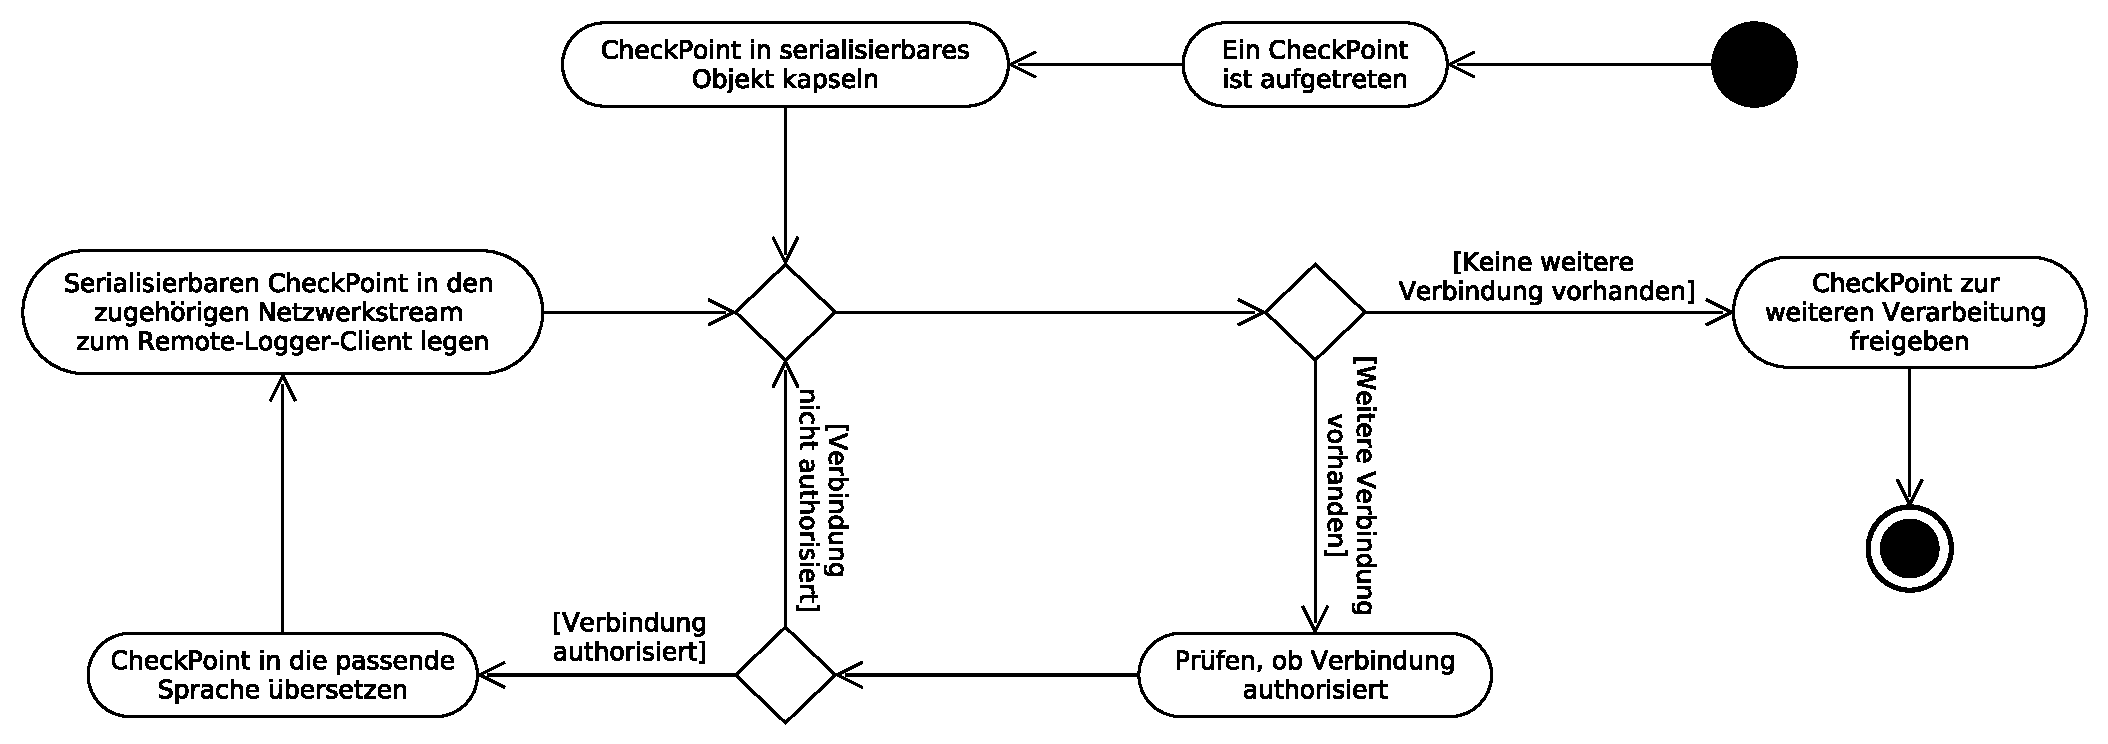
\includegraphics[width=0.9\textwidth]{../img/AD-RemoteLoggerServer.eps}
	\caption{Ablauf am Remote-Logger-Server}
\end{figure}
rjhfedhjcfe lekcvjle

\newpage

\subsubsection{Login des Remote-Logger-Clients am Remote-Logger-Server}
\par Um zu gewährleisten, dass kein unberechtigter Dritter Zugang zu den Logausgaben bekommt, soll ein Login-Mechanismus implementiert werden. Jedoch ist nicht gewünscht, dass der Benutzer des ADITO4-Managers zusätzlich ein zweites Paar Logindaten eingeben muss. Es sollen die gleichen Logindaten verwendet werden, die bereits beim Verbindungsaufbau des Servermangers zum ADITO4-Server benutzt wurden.

\par Es wurde folgende Konzeptgrafik entwickelt:
\begin{figure}[h]
	\vspace{-5px}
	\centering
	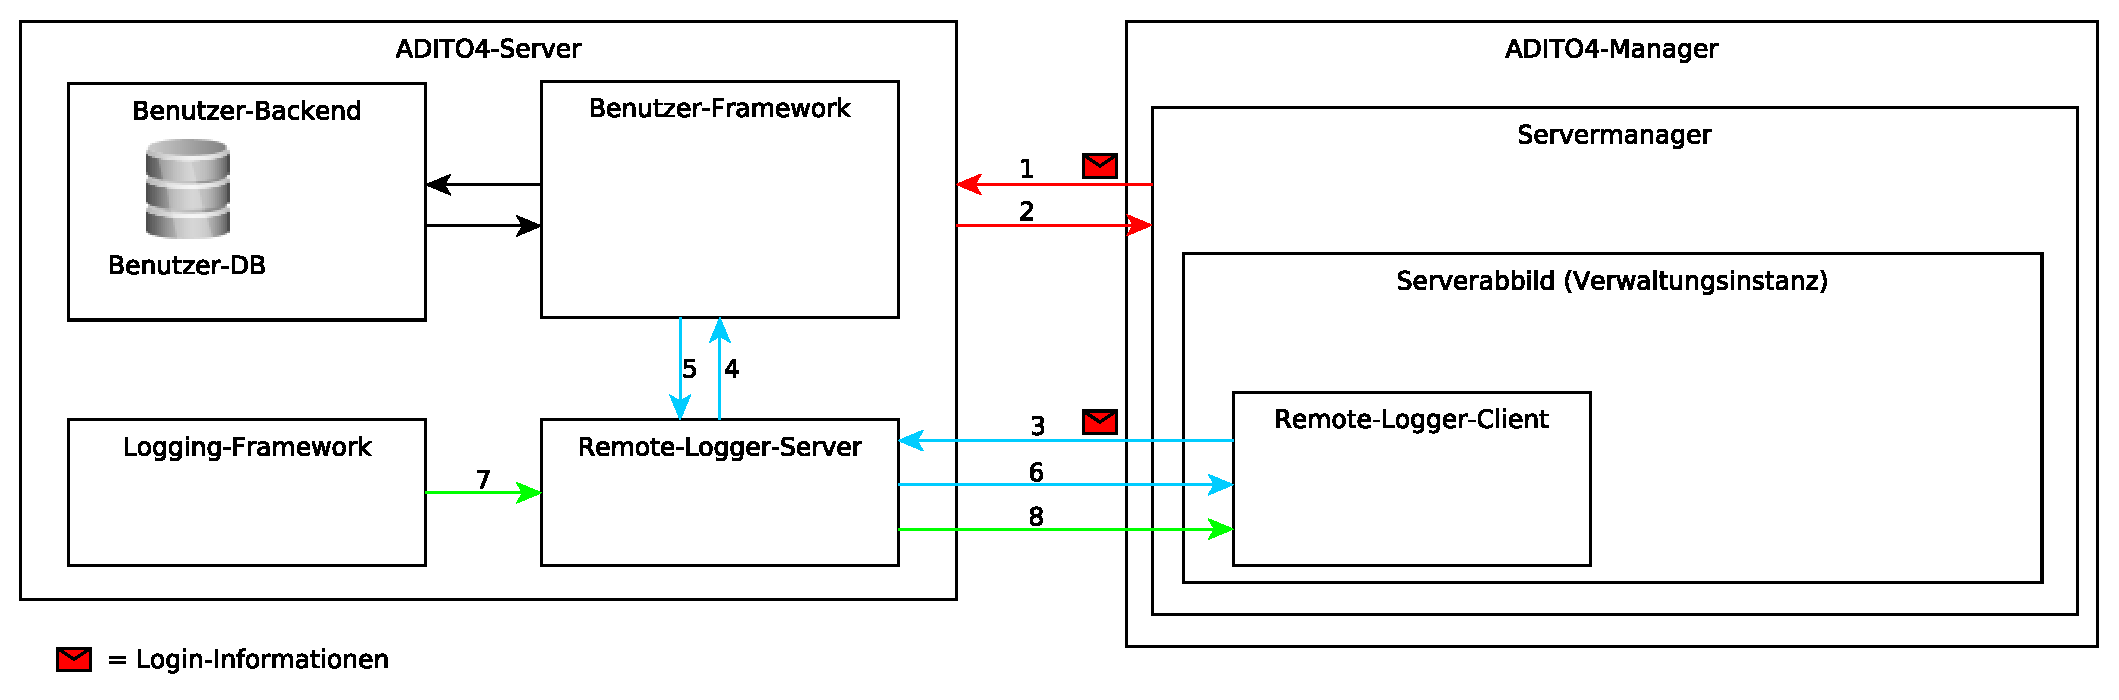
\includegraphics[width=\textwidth]{../img/Kommunikation-ADITO-Server-Manager-Remote-Logger.eps}
	\caption{Login eines Remote-Logger-Clients}
	\label{fig:KommunikationServerManager}
\end{figure}
\vspace{-10px}
\begin{enumerate}[leftmargin=0px]
\item Wenn der Benutzer die Verbindung zu einem neuen ADITO4-Server herstellen möchte, so muss auf der Seite des ADITO4-Managers ein neues Serverabbild erzeugt werden. Nachdem sich der ADITO4-Manager mit dem ADITO4-Server erfolgreich verbunden hat, wird ein Login seitens des ADITO4-Managers benötigt. Hier wird der Benutzer aufgefordert, Logininformationen (symbolisiert durch roten Briefumschlag) einzugeben.
\item Der ADITO4-Server liefert Rückmeldung, ob der Login gültig ist. Wenn ja, wird ein neues Serverabbild erstellt und mit Live-Daten des ADITO4-Servers versorgt. Ansonsten wird die Verbindung sofort getrennt.

\item Nachdem der Servermanager das Abbild des Servers erstellt hat wird, sofern dies der Benutzer wünscht, die Verbindung vom Remote-Logger-Client zum Remote-Logger-Server über den Port 7733 aufgebaut. Sobald diese Verbindung hergestellt ist wird versucht, sich mit den gleichen Informationen einzuloggen, wie es der Servermanager am ADITO4-Server (repräsentiert durch den gleichbleibend roten Briefumschlag).
\item Der Remote-Logger-Server erhält eine Loginanfrage und leitet diese an das Benutzer-Framework des ADITO4-Servers weiter. Nur das kann entscheiden, ob der Login gültig ist.
\item Das Benutzer-Framework des ADITO4-Servers gibt Aufschluss darüber, ob der Login gültig war.
\item Falls die übermittelten Logindaten gültig waren, so wird nun die Verbindung zwischen Remote-Logger-Server und Remote-Logger-Client als \glqq autorisiert\grqq\ betrachtet. CheckPoints dürfen nun gesendet und Kommandos dürfen ausgewertet werden. Falls die Daten ungültig waren, wird die Verbindung seitens des Remote-Logger-Servers mit sofortiger Wirkung aufgelöst.

\item Ein CheckPoint ist am ADITO4-Server aufgetreten. Dieser wird vom Logging-Framework entgegengenommen und unter den Loggern verteilt. So erhält auch der Remote-Logger-Server diese CheckPoints.
\item Der Remote-Logger-Server leitet die aufgetretenen CheckPoints an alle autorisierten Remote-Logger-Clients weiter, sofern die Verbindung autorisiert wurde (Schritt 4 + 5).
\end{enumerate}
\newpage